\chapter{Methodology and involved technologies}
\label{chap:methodology}

\section{Methodology}
\label{section:methodology-spiral}

Due to the researching nature of the main project, it was quite difficult to
establish a fixed set of requirements in the beginning. Therefore, we used
the following system to carry on the process:

\begin{itemize}
  \item Establish a set of main objectives which can be expanded afterwards. The
  final result is the set of objectives which was discussed in Chapter
  \ref{chap:objectives}.
  \item Create a set of use cases based on these discussions.
  \item Create a design which has to be flexible enough to allow the
  introduction of new changes in the future.
  \item Implement a prototype and perform tests.
  \item Do a demonstration.
  \item New elicitation requirements process if necessary.
\end{itemize}

This model follows a spiral model (see Figure \ref{img:spiral}), a software
development process combining elements of both design and prototyping-in-stages, in an effort to combine 
advantages of top-down and bottom-up concepts.

\begin{figure}
 \begin{center}
 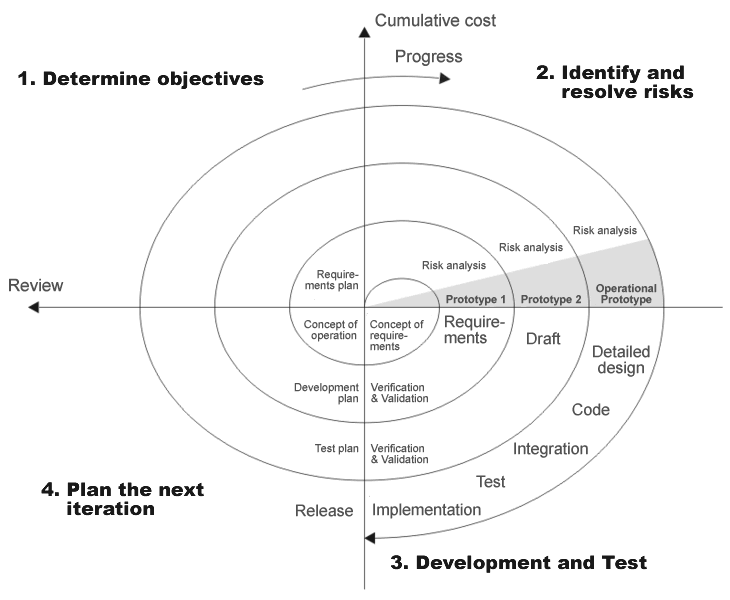
\includegraphics[scale=0.33]{img/spiral_model.png}
 \end{center}
 \caption{\label{img:spiral}Spiral model (Boehm, 1988)}
\end{figure}

Due to the limited extension of this document, it is not possible to explain in
the deserved detail the dynamic followed during the process. But it is
important to stand out at least that the whole process took four iterations
which are briefly explain in the Table \ref{table:iterations}.

%%\begin{center}
\begin{table}[h]
	\small
	\centering
	\begin{tabular}{||r|c|c||}
	\hline \hline
	Iteration & Requirements & Affected components
	\\
	\hline
	\hline 
	1 & Share and retrieve applications & \texttt{RepositoryManager} \& \texttt{PHP
	EUT tools}\\
	\hline
	2 & Tagging & \texttt{TagManagerNode} \& \texttt{TagManagerBackEnd} \\
	\hline
	3 & Searching capabilities & \texttt{RepositoryManager},\\
	  &	\& tagging extensions &\texttt{TagManagerNode} \& \texttt{TagManagerBackEnd}\\
	\hline
	4 & GUI & \texttt{ApplicationManager} \\
	\hline \hline
	\end{tabular}
	\caption{\label{table:iterations}Iterations during the project}
\end{table}
%%\end{center}

We have followed a methodology which can be seen as an Agile software
development methodology \cite{agile-paper}. The concept refers to a group of
software development methodologies based on iterative development, where requirements and  solutions
evolve through collaboration between self-organizing cross-functional teams. 
The term was coined in the year 2001 when the Agile Manifesto
\cite{agile-manifesto} was formulated.

Agile methods generally promote a disciplined project management  process that
encourages frequent inspection and adaptation, a leadership philosophy  that
encourages teamwork, self-organization and accountability, a set of 
engineering best practices that allow for rapid delivery of high-quality 
software, and a business approach that aligns development with customer needs
and company goals. Conceptual foundations of this framework are found in 
modern approaches to operations management and analysis, such as lean 
manufacturing, soft systems methodology, speech act theory (network of 
conversations approach), and Six Sigma.

This methodology fits properly with the researching
nature of the project and the fact that new requirements arise continuously.

%%The documentation which is discussed in the next sections refers to the
%%the final documentation produced as a consequence of all the iterations.

\section{Involved paradigms and technologies}

In this section we will explain briefly the main paradigms and technologies
involved during the achievement of this project.

%%SOA
\subsection{SOA}

Service Oriented Architecture is a paradigm for organizing and utilizing distributed capabilities 
that may be under the control of different ownership domains \cite{soa-principles}.
It provides a uniform means to offer, discover, interact with and use capabilities to produce 
desired effects consistent with measurable preconditions and expectations.
\par
In computing, the term Service-Oriented Architecture expresses a perspective
of software architecture that defines the use of services to support the requirements of software 
users. In an SOA environment, resources on a network are made available as independent services 
that can be accessed without knowledge of their underlying platform implementation.
SOA can also be regarded as a style of Information Systems architecture that
enables the creation of applications that are built by combining loosely coupled and 
inter-operable services.

The main principles behind the SOA paradigm can be summarized as follows:

\begin{itemize}
	\item Reuse
	\item Granularity
	\item Modularity
	\item Composability
	\item Componentization
	\item Interoperability
	\item Compliance to standards (both common and industry-specific) (e.g. Web
Services) 
	\item Services identification and categorization, provisioning and delivery,
and monitoring and tracking
\end{itemize}

\subsubsection{SOAP and Apache Axis}
\label{subsubsec:tech-soap-axis}
SOAP is a lightweight protocol for exchanging structured information in a 
decentralized, distributed environment \cite{w3c-soap-spec}. It is an XML (see
Section \ref{subsec:tech-xml}) based protocol that consists of three parts: an 
envelope that defines a framework for describing what is in a message and how 
to process it, a set of encoding rules for expressing instances of 
application-defined datatypes, and a convention for representing remote 
procedure calls and responses.

The implementation we have used is Apache Axis, it consists of an open source 
Java and C++ implementation of the SOAP server, and various utilities and APIs
for generating and deploying Web service applications. Using Apache Axis, 
it is possible to create interoperable and distributed computing applications.
Axis is developed under the auspices of the Apache Software Foundation.


\subsubsection{ASTRA SOA}
\label{subsubsec:tech-astra-soa}
The ASTRA Service-Oriented Architecture is the backbone of ASTRA 
\cite{astra-soa-white-paper}. It includes the platform for awareness services, 
the ontology, ontology management, context management, service discovery, and 
other necessary modules like the ones developed for this project.

These services are offered by a set of bundles (see Section \ref{subsec:tech-osgi})
that can be grouped into two subsystems from a high level point of view: ASTRA
Node and ASTRA Backend, following a Client-Server model\footnote{There has
been some discussion about the possibility of following a P2P model in ASTRA,
but this is out of the scope of the current implementation.}. Therefore it is
important to distinguish between the local and remote nature connection when 
consuming other bundles services, to take into account the limitations in the
type of objects we can use for our web services interfaces in the case of remote
connections, and to threat properly possible problems in the network.

Below are listed the bundles whose services have been used by the bundles
developed for this project. The dependencies with them are explained in Sections
\ref{subsubsec:connections-rm}, \ref{subsubsec:connections-tmbe},
\ref{subsubsec:connections-tmn} and \ref{subsubsec:connections-am}.

\begin{itemize}
  \item \verb|UserManager|: It is the responsible for managing users and their
  profiles, as well as the management of the user identities. It is executed in
  the Backend.
  \item \verb|CommunityManager|: It is the responsible for providing the
  possibility to define, share and connect virtual community representations in within which
  users can share awareness information. It is executed in the Backend.
  \item \verb|AwarenessManager|: It is the responsible for the connection
  between low level user-system interaction and the high level concepts related to
  them. It is connected with the Rules engine kernel. It is executed in the
  Nodes.
  \item \verb|AwarenessApplicationManager|: It is the responsible for storing
  and managing the local awareness applications. It is executed
  in the Nodes.
  \item \verb|OntologyManager|: It is the responsible for managing, looking-up
  and extending the ontologies. It is executed in the Nodes.
  \item \verb|PersistencyManager|: It is the responsible for providing storage
  functionalities. It is executed in the Backend and the Nodes.
  \item \verb|RemoteFrameworkManager|: It is the responsible for providing
  facilities to consume remote bundles services. It is executed in both subsystems.
  \item \verb|EventsManager|: It is the responsible for providing facilities to
  communicate events between the bundles. It is executed in both subsystems.
\end{itemize}



%Java
\subsection{Java}
Most of the development tasks during the project were coded using Java.
Java is a programming language originally developed by James Gosling at Sun 
Microsystems and released in 1995 as a core component of Sun Microsystems' Java
platform. The language derives much of its syntax from C and C++ but has a
simpler  object model and fewer low-level facilities. Java applications are 
typically compiled to bytecode (class file) that can run on any Java virtual 
machine (JVM) regardless of computer architecture.

The original and reference implementation Java compilers, virtual machines, 
and class libraries were developed by Sun from 1995. As of May 2007, in
compliance  with the specifications of the Java Community Process, Sun made 
available most of their Java technologies as free software under the GNU
General  Public License. Others have also developed alternative implementations
of these Sun technologies, such as the GNU Compiler for Java and GNU Classpath.

Java has significant advantages over other languages and environments  that
make it suitable for just about any programming task.

The advantages of Java are as follows:
\begin{itemize}
  \item Java is easy to learn: Java was designed to be easy to use and is
  therefore easier to write, compile, debug, and learn than other programming
  languages.
  \item Java is object-oriented: This allows us to create modular programs and
  reusable code.
  \item Java is platform-independent: One of the most significant
  advantages of Java is its ability to move easily from one computer system  to
  another. The ability to run the same program on many different systems is 
  crucial to World Wide Web software, and Java succeeds at this by being 
  platform-independent at both the source and binary levels.
\end{itemize}

Because of Java's robustness, ease of use, cross-platform  capabilities and
security features, it has become a language of choice for providing  worldwide
Internet solutions.


%%OSGi
\subsection{OSGi}
\label{subsec:tech-osgi}
%%\subsubsection{What is OSGi?}
OSGi (Open Services Gateway initiative) is a flexible framework, which provides
a standardized environment for service deployment and operation. 
The Framework implements an elegant, complete, and dynamic component
model; something that is missing in standalone Java/VM environments. The
platform is java-based and can be remotely managed.
In Figure \ref{img:osgi} we can see the OSGi layered model.

Applications or components (coming in the form of bundles for deployment) can
be remotely installed, started, stopped, updated and uninstalled without requiring a reboot. 
Bundles are deployed on an OSGi framework, the bundle runtime environment. 
This is not a container like Java Application Servers. It is a collaborative environment. 
Bundles run in the same VM and can actually share code. 
The framework uses the explicit imports and exports to wire up the bundles so they do not have 
to concern themselves with class loading.

\begin{figure}
 \begin{center}
 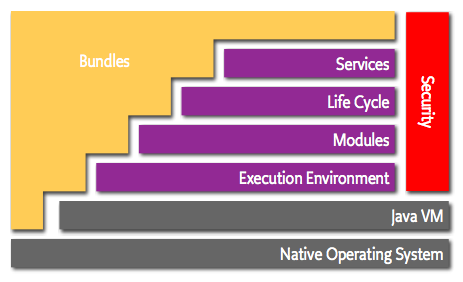
\includegraphics[scale=0.5]{img/layering-osgi.png}
 \end{center}
 \caption{\label{img:osgi}OSGi layered model}
\end{figure}

The original focus was on service gateways but the applicability turned out to be much wider. 
Implementations of the OSGi framework specification are available for a range of different 
environments and device classes, from backend systems via desktops to mobile devices. 
A well-known and popular usage for its flexibility is the Eclipse development framework, 
which is completely based on OSGi. The longest history can OSGi claim on embedded systems, 
where it originally was designed for. Currently Nokia is integrating OSGi technologies into 
their latest phones. 
But also big application servers like IBM WebSphere 6.1 start adapting this technology.

\subsubsection{OSGi-Knopflerfish}
\label{subsubsec:tech-osgi-knopflerfish}

Knopflerfish is a non-profit organization, developing OSGi related material. 
The project provides easy to use open source certified implementation of the OSGi R4 core 
framework specification, as well as related build tools and applications. 
Knopflerfish is available under a BSD style license.

\subsubsection{Why using OSGi in ASTRA?}
OSGi enforces a clean service oriented design approach, with a clear
distinction between interfaces and implementation. 
Services are deployed in bundles, which can be installed, updated and removed
during the runtime of the framework. OSGi is thus ideally suited to realizing
the principles of the SOA paradigm. OSGi also provides an Apache Axis (see
Section \ref{subsubsec:tech-soap-axis}) bundle that allows for automatic 
generation of web service interfaces.

The decision of using the OSGi framework has several severe impacts on the
design  of the functional components.
The most important implications for the component design are summarized here:
\begin{itemize}
	\item Services are de-coupled. A service must not take any assumptions about
the existence and life-cycle of any other service it might want to use (concept
of ``minimal assumptions'').
	\item Services communicate only through their exposed interfaces.
	\item A service must not take any assumptions about the implementation details
	of any other service. 
	The smallest unit for code deployment is a bundle, which might simply contain 
	API's or one or more service implementations.
\end{itemize}

It is worth stressing that OSGi is chosen as a platform, but it is
in no way a requirement by ASTRA to use OSGi. It is used because it offers a
flexible and convenient way of deploying the ASTRA SOA functional components. 
Any ASTRA component can be developed outside OSGi, and made available through a
Web Service interface.

%%Swing
\subsection{Swing}
Swing is a widget toolkit for Java. It is part of Sun Microsystems Java
Foundation Classes (JFC), an API for providing a graphical user interface (GUI)
for Java programs.

Swing was developed to provide a more sophisticated set of GUI components than
the earlier Abstract Window Toolkit. 
It provides a native look and feel that emulates the look and feel of several
platforms, and also supports a pluggable look and feel that allows applications
to have a look and feel unrelated to the underlying platform.

Swing has been used to develop a bundle which implements a GUI to allow the
user to perform all the operations related to the applications and tags
management process. The reason why Swing was chosen is the set of features that
its architecture provides:

\begin{itemize}
	\item Platform independence: Swing is platform independent both in terms of
its expression (Java) and its implementation (non-native universal rendering of
widgets).

	\item Extensibility: Swing is a highly partitioned architecture, which allows
  for the ``plugging'' of various custom implementations of specified framework
  interfaces: Users can provide their own custom implementation(s) of these 
  components to override the default implementations. In general, Swing users 
  can extend the framework by extending existing (framework) classes and/or 
  providing alternative implementations of core components.

	\item Component-oriented:  Swing is a component-based framework. The
	distinction between objects and components is a fairly subtle point: 
	concisely, a component is a well-behaved object with a known/specified 
	characteristic pattern of behaviour. Swing objects asynchronously fire 
	events, have ``bound'' properties, and respond to a well-known set of 
	commands (specific to the component). Specifically, Swing components are  Java
	Beans components, compliant with the Java Beans Component Architecture 
	specifications.

	\item Customizable: Given the programmatic rendering model of the Swing
	framework, fine control over the details of rendering of a component is 
	possible in Swing. As a general pattern, the visual representation of a Swing 
	component is a composition of a standard set of elements, such as a
	``border'', ``inset'', decorations, etc. Typically, users will
	programmatically customize a standard Swing component (such as a
	\verb|JTable|) by assigning specific Borders, Colors, Backgrounds, opacities,
	etc., as the properties of that component. The core component  will then use
	these property (settings) to determine the appropriate renderers to use in
	painting its various aspects. However, it is also completely possible to
	create unique GUI controls with highly customized visual representation.

	\item Configurable: Swing's heavy reliance on runtime mechanisms and indirect 
	composition patterns allows it to respond at runtime to fundamental changes 
	in its settings. For example, a Swing-based application can change its look 
	and feel at runtime. Further, users can provide their own look and feel 
	implementation, which allows for uniform changes in the look and feel of 
	existing Swing applications without any programmatic change to the application
	code.
\end{itemize}

These traits allowed us to fulfill successfully the requirements for the
above-mentioned bundle, which will be explained deeply in Sections
\ref{subsec:am-design} and \ref{subsec:implementation-mvc-swing}.

%XML
\subsection{XML}
\label{subsec:tech-xml}
XML (eXtensible Markup Language) is a general-purpose specification for
creating  custom markup languages. It is classified as an extensible
language,  because it allows the user to define the mark-up elements.

XML's purpose is to aid information systems in sharing structured data, 
especially via the Internet, to encode documents, and to serialize data;  in
the last context, it compares with text-based serialization languages such as 
JSON, YAML, and S-Expressions.

XML's set of tools helps developers in creating web pages but its usefulness
goes well beyond that. XML, in combination with other standards, makes  it
possible to define the content of a document separately from its formatting, 
making it easy to reuse that content in other applications or for other 
presentation environments. Most importantly, XML provides a basic syntax  that
can be used to share information between different kinds of computers, 
applications and organizations without needing to  pass
through many layers of conversion.

XML began as a simplified subset of the Standard Generalized Markup Language 
(SGML), meant to be readable by people via semantic constraints.
Application languages can be implemented in XML. These include XHTML, RSS,
MathML, GraphML, Scalable Vector Graphics, MusicXML, and others. Moreover, XML
is sometimes used as the specification language for such application languages.

XML is recommended by the World Wide Web Consortium (W3C). It is a fee-free 
open standard. The recommendation specifies lexical grammar and parsing 
requirements.

As we will explain in detail in Section
\ref{subsec:implementation-app-adaptation}, XML is the language used to
represent the rules in ASTRA.

%DOM
\subsection{DOM}
\label{subsec:tech-dom}
The Document Object Model (DOM) is a cross-platform and language-independent 
convention for representing and interacting with objects in HTML, XHTML and 
XML documents. Objects under the DOM (also sometimes called ``Elements'') may be
specified and addressed according to the syntax and rules of the programming 
language used to manipulate them. The rules for programming and interacting
with the DOM are specified in the DOM Application Programming Interface (API).


As we will explain in detail in Section
\ref{subsec:implementation-app-adaptation}, DOM was used to access and modify
the rules in ASTRA.


%%Lucene
\subsection{Lucene}
\label{sec:tech-lucene}
Apache Lucene is an open source information retrieval library, originally
created in Java by Doug Cutting. 
It is supported by the Apache Software Foundation and is released under the Apache 
Software License.
Lucene itself is just an indexing and search library and does not contain 
crawling and HTML parsing functionality: it is not an application. 
It allowed us to create a search engine integrated in one of the bundles
(see Sections \ref{subsec:repository-design} and
\ref{subsec:implementation-search-engine}) to offer searching capabilities in
it. The main reasons why Lucene was proposed (and accepted) were:

\begin{itemize}
	\item It is open-source.
	\item It has a great performance.
	\item It is quite flexible and easy to extend if more functionalities are 
	needed in the future.
	\item It is cross-platform.
\end{itemize}


%MySQL
\subsection{MySQL}
\label{subsec:tech-mysql}
MySQL is a relational database management system (RDBMS) very popular in the
free and open source software communities. The program runs as a server
providing multi-user access to a number of databases.

The project's source code is available under terms of the GNU General Public 
License, as well as under a variety of proprietary agreements. MySQL is owned 
and sponsored by a single for-profit firm, the Swedish company MySQL AB, now  a
subsidiary of Sun Microsystems, which holds the copyright of most of the code.

MySQL is commonly used by free software projects which require a full-featured
database management system, such as WordPress, phpBB and other software built 
on the LAMP software stack. It is also used in very high-scale World Wide Web 
products including Google and Facebook.

MySQL is the RDBMS system which is used for taking care of the persistence
in ASTRA.
